\documentclass[11pt,a4paper]{article}

\usepackage[a4paper,margin=20mm]{geometry}
\usepackage{graphicx}
\usepackage{booktabs}
\usepackage{array}
\usepackage{tabularx}
\usepackage{xcolor}
\usepackage{hyperref}
\usepackage{caption}
\usepackage{float}
\usepackage{enumitem}
\usepackage{pdflscape}
\usepackage{tikz}
\usetikzlibrary{arrows.meta,positioning,fit,backgrounds}

\graphicspath{{figures/}}
\hypersetup{
  colorlinks=true,
  linkcolor=blue!55!black,
  urlcolor=blue!55!black,
  pdftitle={A2 Penetration Testing and Threat Modelling Report},
  pdfauthor={Your Name}
}

\setlength{\parindent}{0pt}
\setlength{\parskip}{5pt}
\setlist[itemize]{leftmargin=*,topsep=2pt,itemsep=2pt}
\setlist[enumerate]{leftmargin=*,topsep=2pt,itemsep=2pt}
\captionsetup{font=small,labelfont=bf}
\sloppy

\definecolor{entityblue}{HTML}{DCEFFA}
\definecolor{processgreen}{HTML}{DCFCE7}
\definecolor{storeyellow}{HTML}{FFF3C4}
\definecolor{boundarygray}{HTML}{64748B}
\definecolor{mitpurple}{HTML}{EDE9FE}
\definecolor{mitline}{HTML}{7C3AED}

\newcommand{\evidencefig}[4]{
  \begin{figure}[H]
    \centering
    \includegraphics[width=#3\linewidth,height=#4\textheight,keepaspectratio]{#1}
    \caption{#2}
  \end{figure}
}

\newcommand{\cvss}[2]{\textbf{#1} \hfill \texttt{#2}}

\title{\textbf{[Your Name] -- [Student ID] -- [UnitCode] -- A2}\\
\large Penetration Testing and Threat Modelling Report}
\author{Target VM: Basic Pentesting: 1}
\date{Testing evidence captured on 3 June 2026}

\begin{document}
\maketitle

\section*{GenAI Declaration}
Generative AI was used to help structure this report, organise evidence, create the LaTeX/TikZ diagrams, and draft explanatory text. The penetration testing evidence, screenshots, observed IP addresses, commands, and exploitation results are based on the student's own lab execution. The final report should be reviewed by the student before submission.

\newpage
\section{Q1 Penetration Testing}

\subsection{Executive Summary}
This penetration test assessed the Basic Pentesting: 1 virtual machine on an isolated VirtualBox host-only network. The objective was to identify exploitable weaknesses, document the attack path, and demonstrate the impact using evidence captured from the lab environment.

Three reportable vulnerabilities were identified: WordPress username enumeration, default WordPress administrative credentials leading to remote code execution, and ProFTPD 1.3.3c backdoor command execution. The highest risk issue was the ProFTPD backdoor, which allowed an unauthenticated remote command shell to be opened as root.

The target was successfully compromised. The WordPress path provided application-level access and a \texttt{www-data} shell, while the FTP path demonstrated direct root compromise. Priority remediation should remove ProFTPD 1.3.3c, rebuild the host from trusted media, replace default credentials, restrict administrative access, and harden WordPress against account enumeration and plugin upload abuse.

\subsection{Vulnerability List}
\begin{table}[H]
\centering
\begin{tabularx}{\linewidth}{>{\raggedright\arraybackslash}X c c c >{\raggedright\arraybackslash}p{0.18\linewidth}}
\toprule
\textbf{Vulnerability Name} & \textbf{CVSS 3.0} & \textbf{Severity} & \textbf{Page} & \textbf{Primary Evidence}\\
\midrule
WordPress Username Enumeration & 5.3 & Medium & \pageref{sec:v1} & Figure~\ref{fig:wpscan}\\
Default WordPress Administrative Credentials Leading to RCE & 9.8 & Critical & \pageref{sec:v2} & Figures~\ref{fig:login}--\ref{fig:wwwdata}\\
ProFTPD 1.3.3c Backdoor Command Execution & 9.8 & Critical & \pageref{sec:v3} & Figures~\ref{fig:searchsploit}--\ref{fig:root}\\
\bottomrule
\end{tabularx}
\end{table}

\subsection{Testing Scope and Initial Reconnaissance}
The target was placed on the same host-only network as Kali. Network discovery identified the target at \texttt{192.168.56.101}. Kali used \texttt{192.168.56.102} as the attacking host on the isolated lab network.

\evidencefig{01-target-discovery.png}{Target discovery using \texttt{netdiscover} on the isolated host-only network.}{0.92}{0.42}

Nmap service enumeration found FTP, SSH, and HTTP exposed on the target. The FTP service was ProFTPD 1.3.3c on port 21, SSH was OpenSSH 7.2p2 on port 22, and Apache 2.4.18 was listening on port 80.

\evidencefig{02-nmap-full.png}{Nmap scan identifying FTP, SSH, and HTTP services on the target VM.}{0.82}{0.38}

Directory enumeration on the web service found a hidden \texttt{/secret/} path, including WordPress directories such as \texttt{/wp-admin/}, \texttt{/wp-content/}, and \texttt{/wp-includes/}. Loading the site confirmed that the hidden directory hosted a WordPress blog.

\evidencefig{04-dirb-secret.png}{DIRB output revealing the hidden \texttt{/secret/} WordPress directory.}{0.74}{0.58}

\evidencefig{05-wordpress-site.png}{Hidden WordPress website hosted under \texttt{/secret/}.}{0.86}{0.40}

\subsection{Vulnerability 1: WordPress Username Enumeration}
\label{sec:v1}
\cvss{Severity: Medium, CVSS 5.3}{CVSS:3.0/AV:N/AC:L/PR:N/UI:N/S:U/C:L/I:N/A:N}

\textbf{Vulnerability.} The WordPress site allowed unauthenticated user enumeration. WPScan was run against \texttt{http://vtcsec/secret/} with user enumeration enabled and identified the administrator username \texttt{admin}. No valid session was required to obtain this information.

\textbf{Reproduction Steps.} After DIRB identified the hidden WordPress path, WPScan was executed against \texttt{http://vtcsec/secret/} with user enumeration enabled. The scan output listed \texttt{admin} under identified users.

\evidencefig{06-wpscan-admin.png}{WPScan identifying the WordPress administrator account \texttt{admin}.\label{fig:wpscan}}{0.80}{0.60}

\textbf{Risk.} Username enumeration does not directly provide code execution, but it reduces the difficulty of credential attacks. In this lab, the exposed \texttt{admin} username became immediately useful because the account also used the default password.

\textbf{Recommendation.} Disable or restrict author and REST API user enumeration where possible, avoid predictable administrator usernames, use rate limiting on login and enumeration paths, enable MFA for privileged users, and monitor repeated account discovery attempts.

\textbf{References.} WPScan user documentation and the FIRST CVSS v3.0 calculator were used to classify and score this finding.

\subsection{Vulnerability 2: Default WordPress Administrative Credentials Leading to RCE}
\label{sec:v2}
\cvss{Severity: Critical, CVSS 9.8}{CVSS:3.0/AV:N/AC:L/PR:N/UI:N/S:U/C:H/I:H/A:H}

\textbf{Vulnerability.} The WordPress administrative account accepted the default credential pair \texttt{admin/admin}. After login, administrative access allowed the Metasploit WordPress admin shell upload module to authenticate, upload a malicious plugin payload, and open a Meterpreter session.

\textbf{Reproduction Steps.} The WordPress login page at \texttt{http://vtcsec/secret/wp-login.php} was accessed and the credentials \texttt{admin/admin} were accepted. Metasploit was then configured with the WordPress admin shell upload module, the target URI \texttt{/secret}, username \texttt{admin}, password \texttt{admin}, and Kali's host-only IP as \texttt{LHOST}. Running the module opened a Meterpreter session and \texttt{getuid}/\texttt{id} confirmed execution as \texttt{www-data}.

\evidencefig{07-admin-login.png}{WordPress login attempt using the default administrative credentials.\label{fig:login}}{0.82}{0.42}

\evidencefig{08-dashboard.png}{Successful access to the WordPress administration dashboard.}{0.90}{0.46}

\evidencefig{09-msf-options.png}{Metasploit configuration for the WordPress administrative shell upload exploit.}{0.78}{0.56}

\evidencefig{10-www-data-shell.png}{Shell access obtained as the \texttt{www-data} user.\label{fig:wwwdata}}{0.72}{0.42}

\textbf{Risk.} Administrative WordPress access gives an attacker control over site content, users, themes, and plugins. Because plugin upload can execute server-side PHP, the default credentials led beyond web administration to operating system command execution as \texttt{www-data}.

\textbf{Recommendation.} Remove all default passwords, enforce strong unique passwords, enable MFA, restrict \texttt{wp-admin} access to trusted networks where practical, limit plugin installation privileges, monitor plugin changes, and lock or alert on repeated failed login attempts.

\textbf{References.} Rapid7's WordPress Admin Shell Upload module documentation and the FIRST CVSS v3.0 calculator were used to classify and score this finding.

\subsection{Vulnerability 3: ProFTPD 1.3.3c Backdoor Command Execution}
\label{sec:v3}
\cvss{Severity: Critical, CVSS 9.8}{CVSS:3.0/AV:N/AC:L/PR:N/UI:N/S:U/C:H/I:H/A:H}

\textbf{Vulnerability.} Nmap identified ProFTPD 1.3.3c on port 21. Searchsploit showed known backdoor command execution entries for this version. The Metasploit \texttt{exploit/unix/ftp/proftpd\_133c\_backdoor} module was configured with \texttt{RHOSTS 192.168.56.101}, \texttt{RPORT 21}, payload \texttt{cmd/unix/reverse}, and \texttt{LHOST 192.168.56.102}.

\textbf{Reproduction Steps.} Nmap identified ProFTPD 1.3.3c on TCP port 21. Searchsploit confirmed a matching backdoor command execution exploit. In Metasploit, \texttt{exploit/unix/ftp/proftpd\_133c\_backdoor} was configured with the target IP, FTP port, reverse command shell payload, and Kali host-only IP. Running the module opened a command shell, and \texttt{id}/\texttt{whoami} confirmed root privileges.

\evidencefig{03-searchsploit-proftpd.png}{Searchsploit results for the ProFTPD 1.3.3c backdoor vulnerability.\label{fig:searchsploit}}{0.86}{0.48}

\evidencefig{11-proftpd-msf-options.png}{Metasploit configuration for the ProFTPD 1.3.3c backdoor exploit.}{0.80}{0.58}

\evidencefig{12-proftpd-root-shell.png}{Successful exploitation of the ProFTPD backdoor resulting in root access.\label{fig:root}}{0.80}{0.58}

\textbf{Risk.} This vulnerability is critical because it allows unauthenticated remote command execution. In the lab evidence, the exploit opened a command shell and the \texttt{id} and \texttt{whoami} commands confirmed \texttt{uid=0(root)}. With root access, an attacker could read or alter any file, create accounts, install persistence, or destroy the system.

\textbf{Recommendation.} Remove ProFTPD 1.3.3c immediately and rebuild the system from trusted media. Install only vendor-verified packages, validate file integrity, restrict or disable FTP if it is not required, prefer SFTP/SSH-based file transfer, and investigate the host for persistence or compromise indicators.

\textbf{References.} NIST NVD CVE-2010-20103, VulnHub Basic Pentesting: 1, and the FIRST CVSS v3.0 calculator were used to classify and score this finding.

\newpage
\section{Q2 Threat Modelling}
\subsection{Assumptions}
The model represents a medical wearable diagnosis system. A wearable collects patient activity data and sends motion data to a mobile application over Bluetooth. The mobile application sends API requests to cloud services over the public internet. Cloud services authenticate clinicians, run ML inference, create diagnosis reports, store reports, and record audit events.

\begin{landscape}
\begin{figure}[p]
\centering
\resizebox{0.96\linewidth}{!}{%
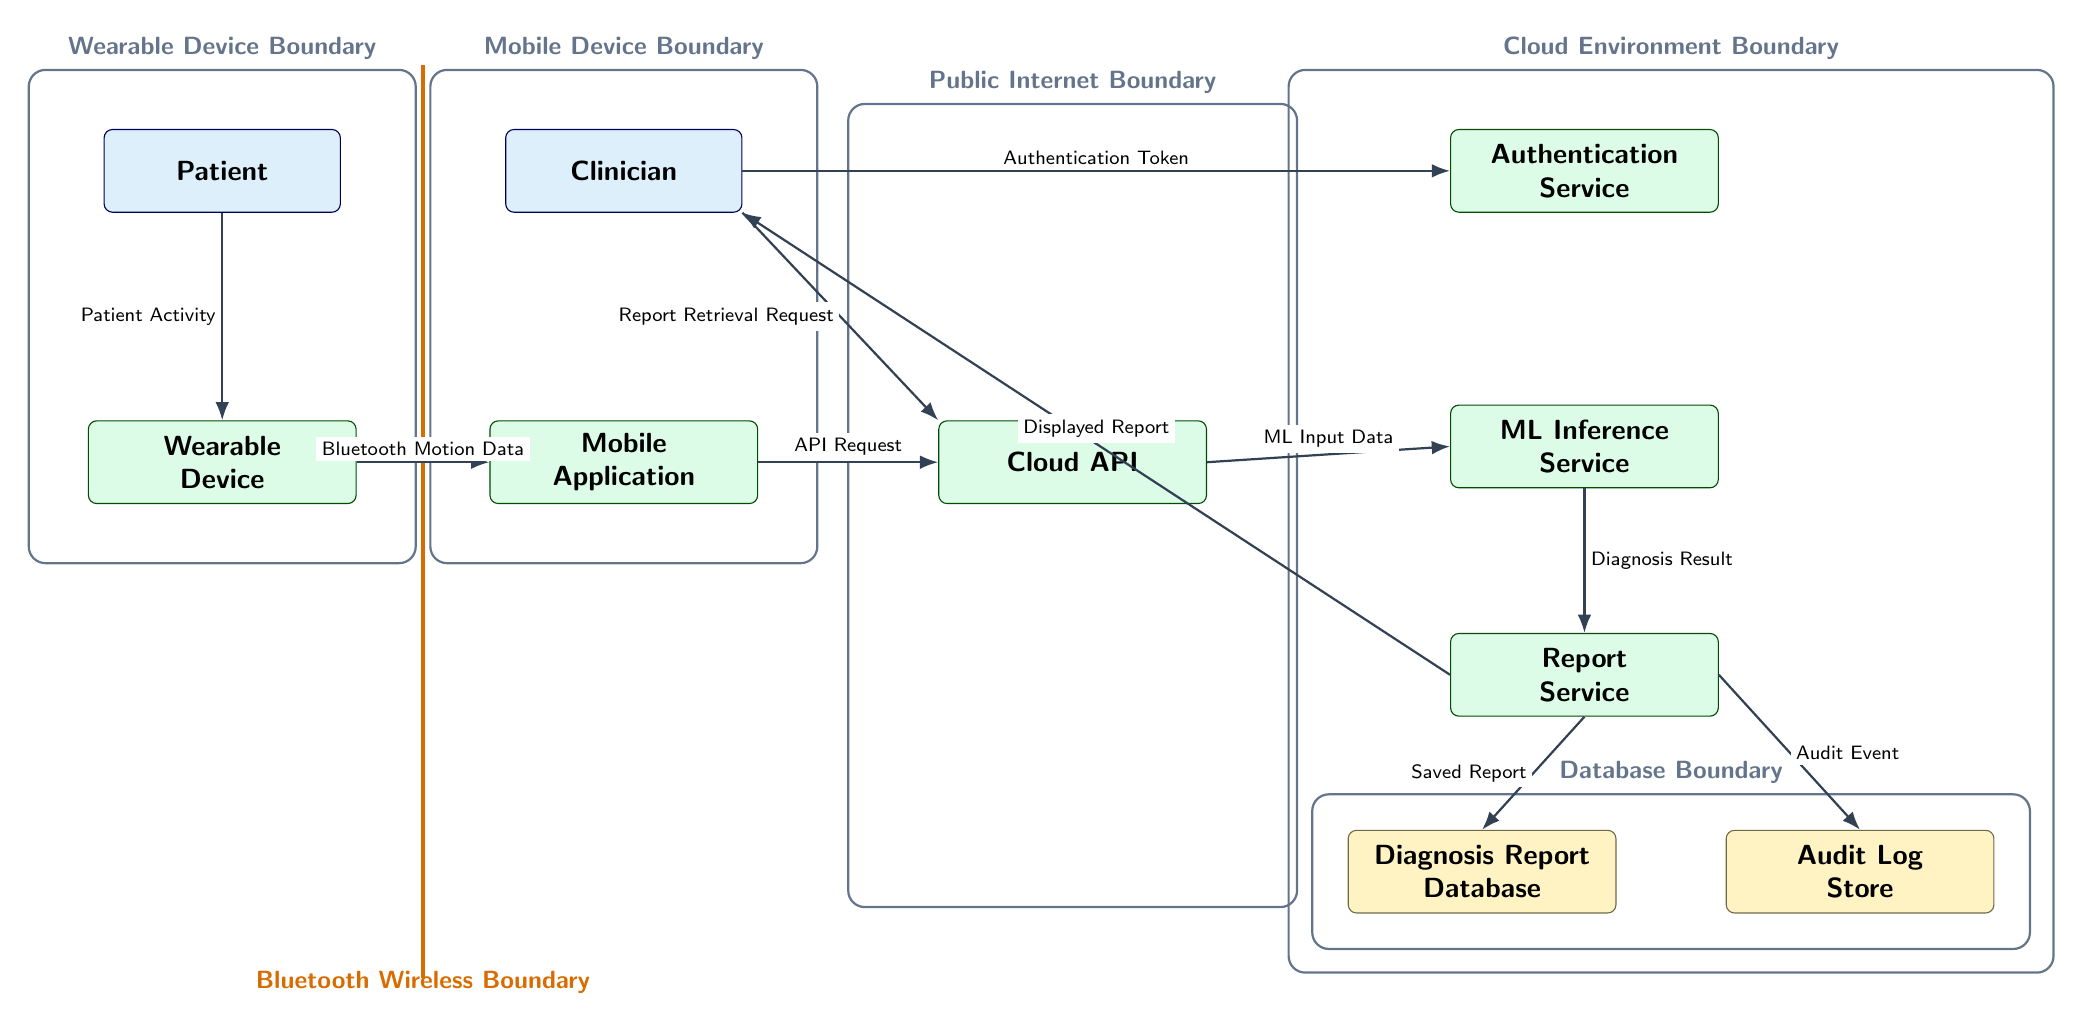
\begin{tikzpicture}[
  >=Latex,
  node distance=1.2cm,
  every node/.style={font=\sffamily},
  entity/.style={draw=blue!35!black, fill=entityblue, rounded corners=3pt, minimum width=3.0cm, minimum height=1.05cm, align=center, font=\sffamily\bfseries},
  process/.style={draw=green!30!black, fill=processgreen, rounded corners=3pt, minimum width=3.4cm, minimum height=1.05cm, align=center, font=\sffamily\bfseries},
  store/.style={draw=yellow!35!black, fill=storeyellow, rounded corners=3pt, minimum width=3.4cm, minimum height=1.05cm, align=center, font=\sffamily\bfseries},
  boundary/.style={draw=boundarygray, rounded corners=6pt, thick},
  flow/.style={->, thick, draw=slategray},
  lab/.style={fill=white, inner sep=2pt, font=\sffamily\scriptsize}
]
\definecolor{slategray}{HTML}{334155}

\node[entity] (patient) at (1.7,10.4) {Patient};
\node[process] (wear) at (1.7,6.7) {Wearable\\Device};
\node[entity] (clinician) at (6.8,10.4) {Clinician};
\node[process] (mobile) at (6.8,6.7) {Mobile\\Application};
\node[process] (api) at (12.5,6.7) {Cloud API};
\node[process] (auth) at (19.0,10.4) {Authentication\\Service};
\node[process] (ml) at (19.0,6.9) {ML Inference\\Service};
\node[process] (report) at (19.0,4.0) {Report\\Service};
\node[store] (db) at (17.7,1.5) {Diagnosis Report\\Database};
\node[store] (audit) at (22.5,1.5) {Audit Log\\Store};

\begin{scope}[on background layer]
\node[boundary, fit=(patient)(wear), inner sep=0.75cm, label={[font=\sffamily\bfseries\small, text=boundarygray]above:Wearable Device Boundary}] (bwear) {};
\node[boundary, fit=(clinician)(mobile), inner sep=0.75cm, label={[font=\sffamily\bfseries\small, text=boundarygray]above:Mobile Device Boundary}] (bmobile) {};
\node[boundary, minimum width=5.7cm, minimum height=10.2cm, anchor=center, label={[font=\sffamily\bfseries\small, text=boundarygray]above:Public Internet Boundary}] (binet) at (12.5,6.15) {};
\node[boundary, fit=(auth)(ml)(report)(db)(audit), inner sep=0.75cm, label={[font=\sffamily\bfseries\small, text=boundarygray]above:Cloud Environment Boundary}] (bcloud) {};
\node[boundary, fit=(db)(audit), inner sep=0.45cm, label={[font=\sffamily\bfseries\small, text=boundarygray]above:Database Boundary}] (bdb) {};
\draw[orange!85!black, ultra thick] (4.25,0.15) -- (4.25,11.75) node[pos=0.02, below, font=\sffamily\bfseries\small] {Bluetooth Wireless Boundary};
\end{scope}

\draw[flow] (patient) -- node[lab, left] {Patient Activity} (wear);
\draw[flow] (wear.east) -- node[lab, above] {Bluetooth Motion Data} (mobile.west);
\draw[flow] (mobile.east) -- node[lab, above] {API Request} (api.west);
\draw[flow] (clinician.east) -- node[lab, above] {Authentication Token} (auth.west);
\draw[flow] (clinician.south east) -- node[lab, left] {Report Retrieval Request} (api.north west);
\draw[flow] (api.east) -- node[lab, above] {ML Input Data} (ml.west);
\draw[flow] (ml.south) -- node[lab, right] {Diagnosis Result} (report.north);
\draw[flow] (report.south) -- node[lab, left] {Saved Report} (db.north);
\draw[flow] (report.east) -- node[lab, right] {Audit Event} (audit.north);
\draw[flow] (report.west) -- node[lab, above] {Displayed Report} (clinician.south east);
\end{tikzpicture}
}
\caption{Original Level 2/3 DFD with trust boundaries. The diagram uses a full landscape page so that wireless, mobile, internet, cloud, and database boundaries remain visually distinct.}
\label{fig:dfd-original}
\end{figure}
\end{landscape}

\subsection{Threat Table and Mitigations}
\begin{table}[H]
\centering
\begin{tabularx}{\linewidth}{>{\raggedright\arraybackslash}p{0.20\linewidth} >{\raggedright\arraybackslash}X >{\raggedright\arraybackslash}p{0.36\linewidth}}
\toprule
\textbf{STRIDE Type} & \textbf{Threat} & \textbf{Mitigation}\\
\midrule
Information Disclosure & Patient motion data, diagnosis reports, or tokens could be exposed over Bluetooth, the public internet, logs, or the report database. & BLE secure pairing, TLS, encryption at rest with KMS, RBAC, and log redaction.\\
Spoofing & An unauthorised user could impersonate a clinician and retrieve patient reports. & MFA, OAuth/OIDC, short-lived tokens, RBAC, and session expiry.\\
Tampering & Motion data or API input could be modified, causing incorrect diagnosis results. & TLS, integrity checks, schema validation, input validation, anomaly detection, and audit logging.\\
Denial of Service & High request volume could exhaust the Cloud API or ML inference service. & API gateway controls, rate limiting, queueing, monitoring, alerting, and capacity scaling.\\
\bottomrule
\end{tabularx}
\end{table}

\begin{landscape}
\begin{figure}[p]
\centering
\resizebox{0.96\linewidth}{!}{%
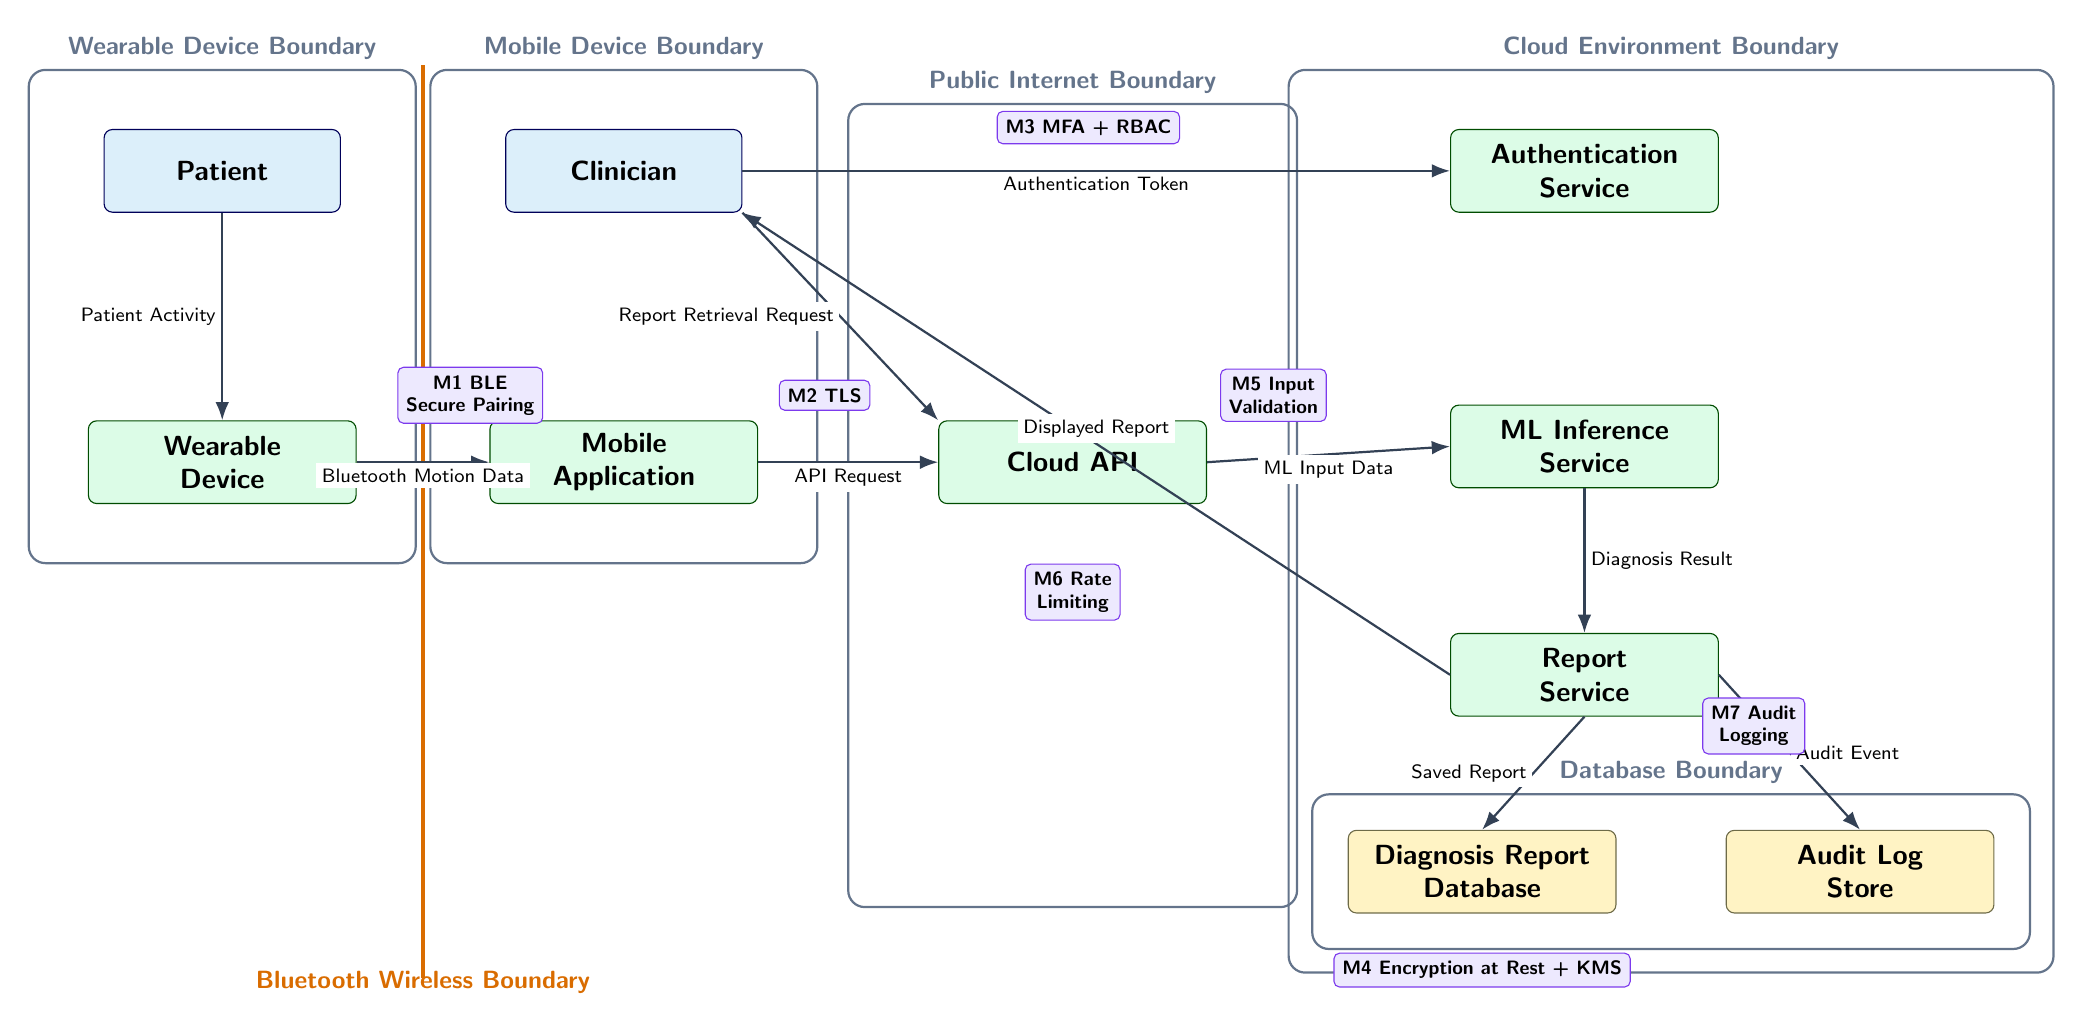
\begin{tikzpicture}[
  >=Latex,
  every node/.style={font=\sffamily},
  entity/.style={draw=blue!35!black, fill=entityblue, rounded corners=3pt, minimum width=3.0cm, minimum height=1.05cm, align=center, font=\sffamily\bfseries},
  process/.style={draw=green!30!black, fill=processgreen, rounded corners=3pt, minimum width=3.4cm, minimum height=1.05cm, align=center, font=\sffamily\bfseries},
  store/.style={draw=yellow!35!black, fill=storeyellow, rounded corners=3pt, minimum width=3.4cm, minimum height=1.05cm, align=center, font=\sffamily\bfseries},
  boundary/.style={draw=boundarygray, rounded corners=6pt, thick},
  flow/.style={->, thick, draw=slategray},
  lab/.style={fill=white, inner sep=2pt, font=\sffamily\scriptsize},
  mit/.style={draw=mitline, fill=mitpurple, rounded corners=2pt, inner sep=3pt, align=center, font=\sffamily\bfseries\scriptsize}
]
\definecolor{slategray}{HTML}{334155}

\node[entity] (patient) at (1.7,10.4) {Patient};
\node[process] (wear) at (1.7,6.7) {Wearable\\Device};
\node[entity] (clinician) at (6.8,10.4) {Clinician};
\node[process] (mobile) at (6.8,6.7) {Mobile\\Application};
\node[process] (api) at (12.5,6.7) {Cloud API};
\node[process] (auth) at (19.0,10.4) {Authentication\\Service};
\node[process] (ml) at (19.0,6.9) {ML Inference\\Service};
\node[process] (report) at (19.0,4.0) {Report\\Service};
\node[store] (db) at (17.7,1.5) {Diagnosis Report\\Database};
\node[store] (audit) at (22.5,1.5) {Audit Log\\Store};

\begin{scope}[on background layer]
\node[boundary, fit=(patient)(wear), inner sep=0.75cm, label={[font=\sffamily\bfseries\small, text=boundarygray]above:Wearable Device Boundary}] (bwear) {};
\node[boundary, fit=(clinician)(mobile), inner sep=0.75cm, label={[font=\sffamily\bfseries\small, text=boundarygray]above:Mobile Device Boundary}] (bmobile) {};
\node[boundary, minimum width=5.7cm, minimum height=10.2cm, anchor=center, label={[font=\sffamily\bfseries\small, text=boundarygray]above:Public Internet Boundary}] (binet) at (12.5,6.15) {};
\node[boundary, fit=(auth)(ml)(report)(db)(audit), inner sep=0.75cm, label={[font=\sffamily\bfseries\small, text=boundarygray]above:Cloud Environment Boundary}] (bcloud) {};
\node[boundary, fit=(db)(audit), inner sep=0.45cm, label={[font=\sffamily\bfseries\small, text=boundarygray]above:Database Boundary}] (bdb) {};
\draw[orange!85!black, ultra thick] (4.25,0.15) -- (4.25,11.75) node[pos=0.02, below, font=\sffamily\bfseries\small] {Bluetooth Wireless Boundary};
\end{scope}

\draw[flow] (patient) -- node[lab, left] {Patient Activity} (wear);
\draw[flow] (wear.east) -- node[lab, below] {Bluetooth Motion Data} (mobile.west);
\draw[flow] (mobile.east) -- node[lab, below] {API Request} (api.west);
\draw[flow] (clinician.east) -- node[lab, below] {Authentication Token} (auth.west);
\draw[flow] (clinician.south east) -- node[lab, left] {Report Retrieval Request} (api.north west);
\draw[flow] (api.east) -- node[lab, below] {ML Input Data} (ml.west);
\draw[flow] (ml.south) -- node[lab, right] {Diagnosis Result} (report.north);
\draw[flow] (report.south) -- node[lab, left] {Saved Report} (db.north);
\draw[flow] (report.east) -- node[lab, right] {Audit Event} (audit.north);
\draw[flow] (report.west) -- node[lab, above] {Displayed Report} (clinician.south east);

\node[mit] at (4.85,7.55) {M1 BLE\\Secure Pairing};
\node[mit] at (9.35,7.55) {M2 TLS};
\node[mit] at (12.7,10.95) {M3 MFA + RBAC};
\node[mit] at (15.05,7.55) {M5 Input\\Validation};
\node[mit] at (12.5,5.05) {M6 Rate\\Limiting};
\node[mit] at (17.7,0.25) {M4 Encryption at Rest + KMS};
\node[mit] at (21.15,3.35) {M7 Audit\\Logging};
\end{tikzpicture}
}
\caption{Level 2/3 DFD with mitigations added. Mitigation labels are positioned close to the protected flow or component while leaving trust boundaries readable.}
\label{fig:dfd-mitigated}
\end{figure}
\end{landscape}

\newpage
\section*{References}
\begin{itemize}
  \item NIST National Vulnerability Database. CVE-2010-20103: ProFTPD 1.3.3c backdoor. \url{https://nvd.nist.gov/vuln/detail/CVE-2010-20103}
  \item Rapid7. WordPress Admin Shell Upload Metasploit module. \url{https://www.rapid7.com/db/modules/exploit/unix/webapp/wp_admin_shell_upload/}
  \item WPScan Team. WPScan User Documentation. \url{https://github.com/wpscanteam/wpscan/wiki/WPScan-User-Documentation}
  \item FIRST. Common Vulnerability Scoring System v3.0 Calculator. \url{https://www.first.org/cvss/calculator/3.0}
  \item Oracle VirtualBox Documentation. \url{https://www.virtualbox.org/manual/}
  \item Kali Linux Documentation. Import pre-made Kali VirtualBox VM. \url{https://www.kali.org/docs/virtualization/import-premade-virtualbox/}
  \item VulnHub. Basic Pentesting: 1. \url{https://www.vulnhub.com/entry/basic-pentesting-1,216/}
\end{itemize}

\end{document}
